% !TEX root = ../my-thesis.tex
%
\chapter{Introduction}
\label{sec:intro}

\cleanchapterquote{
	\textgreek{Δέδυκε μὲν ἀ σελάννα}\\
	\textsuperscript{The moon and the Pleiades}\\
	\textgreek{καὶ Πληΐαδες, μέσαι δέ}\\
	\textsuperscript{have set, it is}\\
	\textgreek{νύκτες, πάρα δ' ἔρχετ' ὤρα,}\\
	\textsuperscript{midnight, time is passing,}\\
	\textgreek{ἔγω δὲ μόνα κατεύδω.}\\
	\textsuperscript{but I sleep alone.}\\
}{Sappho, `The Midnight Poem'}{(c. 600 BC)}

% ---------------------------------------
\section{From seven sisters to a powerhouse of astronomy}
\label{sec:intro:intro}

In all of astronomy, few objects have retained relevance throughout the centuries as much as open clusters (OCs). Easily visible to the naked eye, the Pleiades has been observed since at least the dawn of civilisation CITEME, along with a handful of other OCs visible without a telescope. In the present day, the now thousands of known OCs are a key tool in modern astronomy for understanding stellar and galactic evolution.

Star clusters are formed when clouds of cold molecular gas collapse due to gravity, forming stars. Sometimes, when star formation occurs densely enough, these stars fall further into gravitationally bound clusters that can survive in the galactic disk for as long as $\sim 10^9$~years \citep{lada_embedded_2003,portegies_zwart_young_2010}. It is this property of the formation of OCs that makes them so useful: all stars in an OC will have the same age and initial composition, allowing parameters of the overall group of stars to be measured significantly more precisely than when studying stars in isolation. 

For instance, when a parameter such as the distance of member stars can simply be averaged over all member stars, then the precision of the mean distance of an OC (and hence the distance to all of its member stars) will be a factor $\sqrt{n}$ more precise than the distance to any individual star. Alternatively, when a property such as chemical composition is highly time consuming to derive, it can be derived for a fraction of stars in an OC and be applied to all stars in a cluster.

The ease of studying stellar astrophysics with OCs results in OCs having an extremely wide range of scientific use cases. For instance, OCs are used as testing grounds for stellar evolution models CITEME, as tracers of galactic structure \citep{cantat-gaudin_painting_2020,castro-ginard_milky_2021}, or even as calibrators of cepheid variable stars \citep{medina_revisited_2021}, which are an essential first rung on the cosmic distance ladder and are vital in the derivation of the cosmological parameters of the universe. It is somewhat of a cliché to describe OCs as `the laboratories of stellar evolution', but it really is true: OCs are a fantastic way to observe stars of a given age and composition across a broad range of masses, and to do so with orders of magnitude more precision than when studying isolated field stars.

The best part of the modern story of the OC's contribution to astrophysics comes with the \gaia\ satellite, however. In just five years since its first full data release \citep{brown_gaia_2018}, \gaia\ has revolutionised the study of our galaxy, including the study of OCs; with dozens of papers reporting thousands of new objects \citep[e.g.][]{liu_catalog_2019,castro-ginard_hunting_2019,castro-ginard_hunting_2020,castro-ginard_hunting_2022}, and a number of works deriving dramatically improved parameters and members for OCs in the Milky Way \citep[e.g.][]{cantat-gaudin_gaia_2018,tarricq_3d_2020}. Arguably, there has never been a better time to do science with OCs, owing to the incredible quantity and quality of data that \gaia\ has provided.

There is, however, a catch. Even though the Milky Way is estimated to contain as many as $10^5$ OCs \citep{dias_new_2002}, there are still only a few thousand currently known in the literature -- representing a small fraction of the total number of OCs in our galaxy. It has been shown that the census of OCs is incomplete within even 1~kpc from the Sun \citep[e.g.][]{castro-ginard_new_2018}, and the extent of the remaining incompleteness is unknown. Worse still, it has been shown that many of the OCs catalogued previously in the literature may not exist \citep{cantat-gaudin_clusters_2020,piatti_catching_2023}, with it being largely unknown which OCs are or are not real. The many fantastic uses of OCs in other areas of astronomy are contingent on a reliable, accurate, and complete census of OCs; and the many current caveats with the census of OCs limit the science potential of these fantastic objects in a time when we have more available data with which to study them than ever before.

% TODO: this paragraph is too weak
In this thesis, I will present solutions to a number of the current issues with the OC census in the era of \gaia, using a range of data analysis and parameter inference techniques. I will then use these techniques to create the largest census of OCs to date and derive a range of parameters for these OCs. With this thesis, I also hope to present methods that could continue to be used to maximise the quality of the OC census for the coming decade of \gaia\ data releases -- as well as for whatever instruments supercede \gaia\ in the future.

Before launching into the chapters detailing my work over the past three and a half years, it is worth first conducting an overview of the science behind OCs in the introduction to this thesis. In Sect.~\ref{sec:intro:history}, I will discuss the history of OC observations up to before the release of \gaia\ DR2 in 2018, as well as briefly discussing the techniques and results from pre-\gaia\ observations. Section~\ref{sec:intro:gaia} will then discuss the stunning data of \gaia\ and how it has already thoroughly revolutionised our understanding of OCs in just a handful of years. Finally, Sect.~\ref{sec:intro:theory} will briefly discuss some key pieces of theory surrounding the structure, dynamics, and lifetime of OCs, providing a good background on our theoretical knowledge of OCs that will assist with the reading of this thesis.

The nomenclature and definition of star clusters varies throughout the literature. Hence, in the next section, I will quickly discuss a definition of OCs that I will adopt throughout the rest of this work.


% ---------------------------------------
\section{The definition of an open cluster}
\label{sec:intro:definition}

\begin{figure}[tb]
	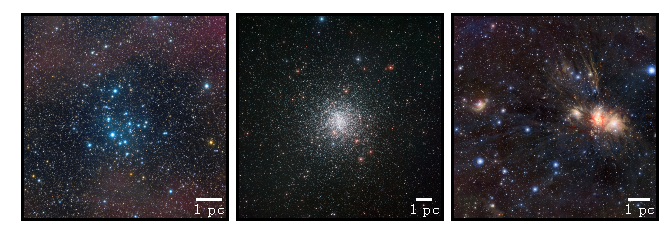
\includegraphics[width=\textwidth]{fig/c1/oc_gc_mg_comparison.pdf}
	\caption[A visual comparison between the three main types of star cluster found in the Milky Way]{A visual comparison between the three main types of star cluster found in the Milky Way. \emph{Left:} the open cluster NGC~2547. \emph{Middle:} the globular cluster M~4. \emph{Right:} the moving group/OB association Monoceros~R2. All images contain a scale in the bottom right showing a length of 1~pc at the distance of each cluster. \emph{Credit, left to right:} ESO / J. Pérez; ESO; ESO / J. Emerson / VISTA. }
	\label{fig:intro:definition:comparison}
\end{figure}

There are many different types of star cluster in the universe. Avoiding confusion when talking about star clusters is important, particularly since observers and theorists often use very different nomenclature. Definitions of star clusters can differ significantly between galactic and extra-galactic astronomy. I will use the following definitions consistently throughout this thesis for clarity.

This thesis will almost exclusively discuss clusters observed in the Milky Way, which are traditionally divided into three broad categories. This thesis will primarily discuss open clusters (OCs), although I will also touch on globular clusters (GCs) and moving groups (MGs). I differentiate between these three types of cluster approximately as follows, matching the observational definitions in \cite{portegies_zwart_young_2010}.

OCs are gravitationally bound clusters with a typical age of around 100~Myr, although some are older than 1~Gyr and some are as young as 0.1~Myr. OCs have masses of typically no greater than $10^4$~\MSun and may be made up of a few dozen to a few thousand stars, with a typical minimum being ten stars. OCs are remants of recent star formation and are hence predominantly located in the galactic disk where the star formation rate is highest. Most OCs have a size of around 3 to 10~pc. Other than some exceptions, OCs contain a single population of stars. 

GCs are much older and more massive gravitationally bound clusters, with ages typically greater than 10~Gyr and masses typically greater than $10^5$~\MSun. The largest GCs can contain a million stars or more. GCs have a typical size around 10 to 20~pc. GCs tend to reside in the galactic bulge or in the galactic halo. Many GCs contain multiple populations of stars. Almost all OCs have masses significantly lower than the typical present day mass of GCs, although observations of a handful of young massive clusters in the Milky Way such as Westerlund~1 (sometimes also referred to as `super star clusters') as well as observations of galaxies with more active star formation suggest that the highest mass star clusters will be long-lived and will evolve into GCs. However, this is not the case for almost all OCs that I will study in this thesis, as the only young massive clusters in the Milky Way are generally distant, heavily reddened, and outside of the reach of the visual-band observations of the \gaia\ telescope.

On the other hand, MGs are of a similar mass and number count to OCs, except they are not gravitationally bound. Due to this, they disperse much more quickly, and hence often have much younger ages. MGs have the widest definition, and encompass any group of stars that are comoving and coeval, but are specifically \emph{not} gravitationally bound. Some MGs are also referred to as `OB associations' in the literature, due to them often containing a number of young, high mass O and B stars. 

\begin{table}[tb]
	\begin{tabularx}{\textwidth}{l | X | X | X | X}
		\hline\hline
		Type & Bound? & Age & Mass & Location \\
		\hline
		Open cluster (OC)   & Weakly & $\lesssim 1$ Gyr & $\lesssim 10^4$ \MSun & Disk \\
		Globular cluster (GC)   & Strongly & $\gtrsim 10$ Gyr & $\gtrsim 10^5$ \MSun & Halo/Bulge \\
		Moving group (MG)   & No & $\lesssim 50$ Myr & $\lesssim 10^3$ \MSun & Disk\\
		\hline
	\end{tabularx}
	\caption{Approximate definitions for the three types of star cluster that will be discussed in this thesis.\label{tab:intro:definition:definition}}
\end{table}

These definitions are summarised in Table~\ref{tab:intro:definition:definition} and compared visually in Fig.~\ref{fig:intro:definition:comparison}. The figure shows three clusters; NGC~2547, M~4, and Monoceros~R2. NGC~2547 is a sparser OC that has a clear core of young blue stars at its center, about $\sim 1$~pc across. On the other hand, despite being only slightly larger, the GC M~4 clearly contains significantly more stars. The stars in M~4 are older, with the cluster having a whiter, redder appearance. Finally, the MG Monoceros~R2 is simply a group of young blue stars, with no discernible core. 





% ---------------------------------------
\section{The history of open cluster observations up until the present day}
\label{sec:intro:history}

In this chapter, I present a literature review of how open clusters have been observed up until the present day, including many key results and touching on a number of still-unanswered questions.

\subsection{The pre-\gaia\ history of open cluster observations}
\label{sec:intro:history:history}

% Plot of the pleiades
\begin{figure}[tb]
	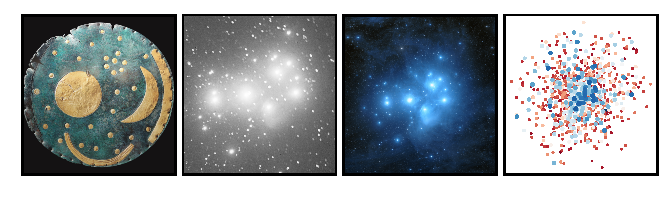
\includegraphics[width=\textwidth]{fig/c1/pleiades.pdf}
	\caption[The Pleiades as depicted throughout history]{The Pleiades, as depicted throughout history and showing the clear improvements in astronomical data gathering over time. \emph{Left:} the Nebra Sky Disc, depicting the Pleiades with its seven naked-eye visible stars in the upper center. The disc was discovered in 1999 in northern Germany and is dated to between 1800-1600 BC. \emph{Middle left:} the Pleiades, as imaged in 1909 with Wolf's Doppelastrograph at the Landessternwarte Heidelberg-Königstuhl. \emph{Middle right:} the Pleiades, as imaged by Hubble. \emph{Right:} the $\sim$1000 member stars for the Pleiades extracted from \gaia\ DR2 data and isolated from field stars by \cite{cantat-gaudin_characterising_2018}. Each star is represented by a point scaled by its magnitude and coloured according to its $BP-RP$ colour. \emph{Image credits:} Frank Vincentz; Heidelberg Digitized Astronomical Plates; Davide De Martin / NASA/ESA Hubble.}
	\label{fig:intro:history:pleiades}
\end{figure}

While the results of this thesis are entirely derived using data from \gaia\ , to truly understand just how groundbreaking the current data of the \gaia\ satellite is, it is worth first briefly reviewing the history of OC observations.

Our ability to observe OCs has progressed incredibly far throughout the history of astronomy (Fig.~\ref{fig:intro:history:pleiades}). The invention of the refracting telescope allowed for early astronomers such as Galileo to observe that OCs and GCs are in fact clusters of many stars, as opposed to being dispered single sources as previously believed from unaided observations. It was, however, the invention and widespread adoptation of the reflecting telescope in the 17\textsuperscript{th} and 18\textsuperscript{th} centuries that led to catalogues of clusters like we use today.

% Plot of catalogues of OCs
\begin{figure}[tb]
	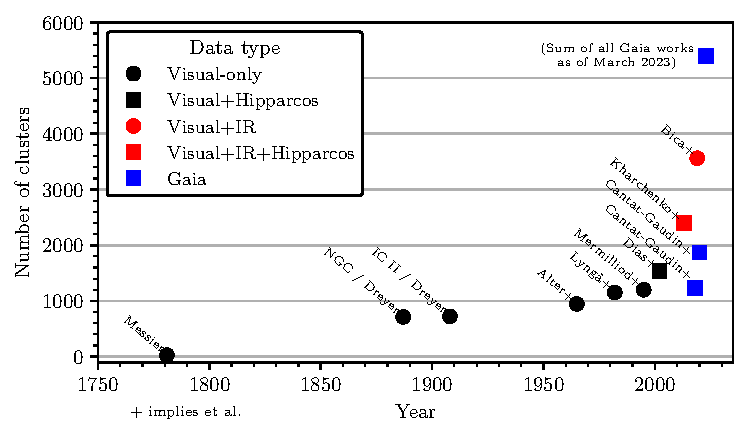
\includegraphics[width=\textwidth]{fig/c1/catalogues.pdf}
	\caption[The size of OC catalogues over time]{The size of OC catalogues over time. After the initial rise in the size of catalogues due to the advent of reflecting telescopes in the 18\third\ and 19\third\ centuries, it was not until the past 25 years and the advent of large-scale astrometric and IR datasets that the OC census significantly increased in size. \\
	{\footnotesize N.B.: this is not an exhaustive plot of all catalogues, and a number of old catalogues such as \cite{herschel_catalogue_one_1786} and \cite{herschel_general_catalogue_1864} without digitised versions are not included.}}
	\label{fig:intro:history:catalogues}
\end{figure}

The power of reflecting telescopes allowed astronomers to scan the sky to signficantly greater depth, searching for clusters of stars and discovering many new objects in the process \citep[e.g.][]{herschel_catalogue_one_1786}, with the number of known OCs jumping from a few dozen to around 700 in a little over a century. Figure~\ref{fig:intro:history:catalogues} shows the evolution in size of OC catalogues over time, showing the peak of around 700 clusters by the turn of the 20\textsuperscript{th} century. Many of the OCs known and catalogued by astronomers at this point were some of the largest and most scientifically useful, with many of these OCs (especially those in the NGC catalogue) being some of the most frequently studied objects even today. 

% Plot of CMDs of OCs
\begin{figure}[tb]
	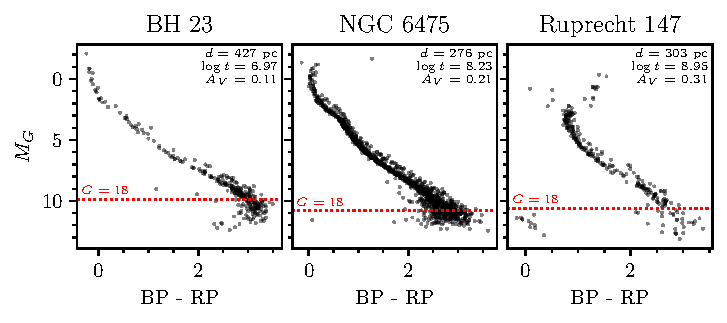
\includegraphics[width=\textwidth]{fig/c1/cmd_comparison.pdf}
	\caption[A comparison of the CMDs of a number of nearby OCs]{A comparison of the CMDs of a number of nearby OCs, using membership lists from later in this thesis in Sect.~\ref{sec:census} and plotted with their absolute magnitude $M_G$ against colour $BP - RP$. The OCs are plotted from left to right in order of increasing age, with their distance $d$, logarithmic age $\log t$ and extinction $A_V$ shown in the top right. The dashed red line indicates the approximate 100\% completeness limit of these OC membership lists, with sources fainter than an apparent magnitude of $G=18$ frequently being missed and often having under-estimated $BP-RP$ colours. BH~23 is less than 10~Myr old and has almost no main sequence turn off; NGC~6475 is over 100~Myr old and has a clear turn off; Ruprecht~147 is around 1~Gyr old and even has a clear population of white dwarf stars.}
	\label{fig:intro:history:cmds}
\end{figure}

The 20\textsuperscript{th} century saw improvements to data gathering and techniques, with early photometric and spectroscopic methods allowing authors such as \cite{rosenberg_uber_zusammenhang_1910} and \cite{hertzsprung_ueber_verwendung_1911} to plot the brightness of the stars in the Pleiades and the Hyades against their spectral features, noticing for the first time that the brightness of stars is related to their colour and spectral features. \cite{russell_relations_spectra_1914} derived the absolute magnitude of stars in the Hyades and ploted this against an early spectral analogue of the temperature of its member stars, plotting the luminosity of stars against their temperature for the first time and inventing `Hertzsprung-Russell' or `colour-magnitude' diagrams (CMDs), a type of plot used extensively in the present day as an essential tool to understand stellar evolution. Later, the differences in CMDs between different clusters were noticed and was interpreted as being a difference in age between the clusters, allowing for the ages of stars within star clusters to be estimated and beginning the foundation of our knowledge of stellar evolution \ref{fig:intro:history:cmds}.

While the 20\textsuperscript{th} century saw huge strides in our understanding of stars and star clusters, the size of OC catalogues went relatively unchanged (Fig.~\ref{fig:intro:history:catalogues}). It was not until the 1990s and the arrival of new methodologies that the OC census itself has begun its largest upheaval since the widespread adoptation of reflecting telescopes more than 200 years prior.

The launch of the \emph{Hipparcos} satellite and subsequent data releases \citep{perryman_hipparcos_1997} produced a catalogue of around 10$^5$ sources with five-parameter milliarcsecond-precision astrometry. OCs stand out as overdensities in \emph{Hipparcos} data, in particular in proper motions, as OCs are comoving groups of stars that often have different velocities to background field sources. This new data allowed works such as \cite{platais_search_1998} to discover a number of new OCs, with many being small objects near to the Sun that evaded detection with only two-dimensional visual observations. 

This resulted in the catalogue of \cite{dias_new_2002} including over 300 more objects than the roughly ten years prior catalogue of \cite{mermilliod_database_1995} (Fig.~\ref{fig:intro:history:catalogues}), representing the largest 
major jump in the size of the OC census in over a century, in addition to the much more accurate mean cluster proper motions and parallaxes provided by \emph{Hipparcos}. However, this was just the beginning, and more new science was to come.

The release of the Two Micron All Sky Survey \citep[2MASS,][]{skrutskie_two_2006} in the 2000s provided the next major jump in data availability for furthering OC science. The infrared (IR) data of 2MASS and its associated catalogue of 471 million point sources allowed works such as \cite{froebrich_systematic_2007} to uncover over a thousand new OC candidates in the galactic disk, using IR data to peer through insterstellar dust and unveil many previously-obscured objects for the first time. In addition, works around this time began to make increasing use of advances in computing power, with works such as \cite{froebrich_systematic_2007} using automated retrieval to extract cluster candidates. CITEME MORE REFERENCES HERE

Work predominantly with IR data culminated in the catalogue of \cite{kharchenko_global_2013}, who derived homoegeneous membership lists, ages, extinctions, distances, proper motions, radii, and many other parameters for a total of 3006 clusters, 2399 of which are OCs or probable OCs. % Until \gaia\ DR2, the catalogue of \cite{kharchenko_global_2013} remained the largest catalogue of OCs.

In around 20 years, the OC census more than doubled in size between the work of \cite{mermilliod_database_1995} to the work of \cite{kharchenko_global_2013}. This unprecedented shift represented the first time that the OC census had been significantly expanded in over a century, with improved datasets offering significantly better measurements of more clusters than ever before. 

Yet seismic shift in cluster catalogues brought about by IR datasets and \emph{Hipparcos} was scarcely the beginning of the modern revolution in studies of OCs. \gaia's first full data release in 2018, DR2 \citep{brown_gaia_2018}, sparked the next revolution in the census of OCs.

\subsection{The \gaia\ revolution}
\label{sec:intro:history:gaia}

For almost all of the history of astronomy, our view of the Milky Way has been strictly two-dimensional. Observing a three-dimensional galaxy in two dimensions is inherently limiting; it took until the 20\third century to even discover that galaxies are separate from the Milky Way. Although astrometric parameters like parallaxes have been measured for stars for over a century, and can be used to view the stars of galaxy in three dimensions, these datasets have always been limited to a few hundred or thousand stars until now.

\gaia\ is a space-based telescope launched in 2013 that aims to measure a wealth of parameters to an unprecedented level of precision for around $10^9$ stars. \gaia\ is measuring precise positions, proper motions, parallaxes, and photometry for its full sample of stars, and also measures radial velocities and low-resolution spectra for a brighter subsample of sources \citep{gaia_collaboration_gaia_2016}. It is the incredible scale and precision of \gaia\ data that sets it apart from any previous datasets.

% Plot of hipparcos vs. gaia astrometric accuracy
\begin{figure}[tb]
	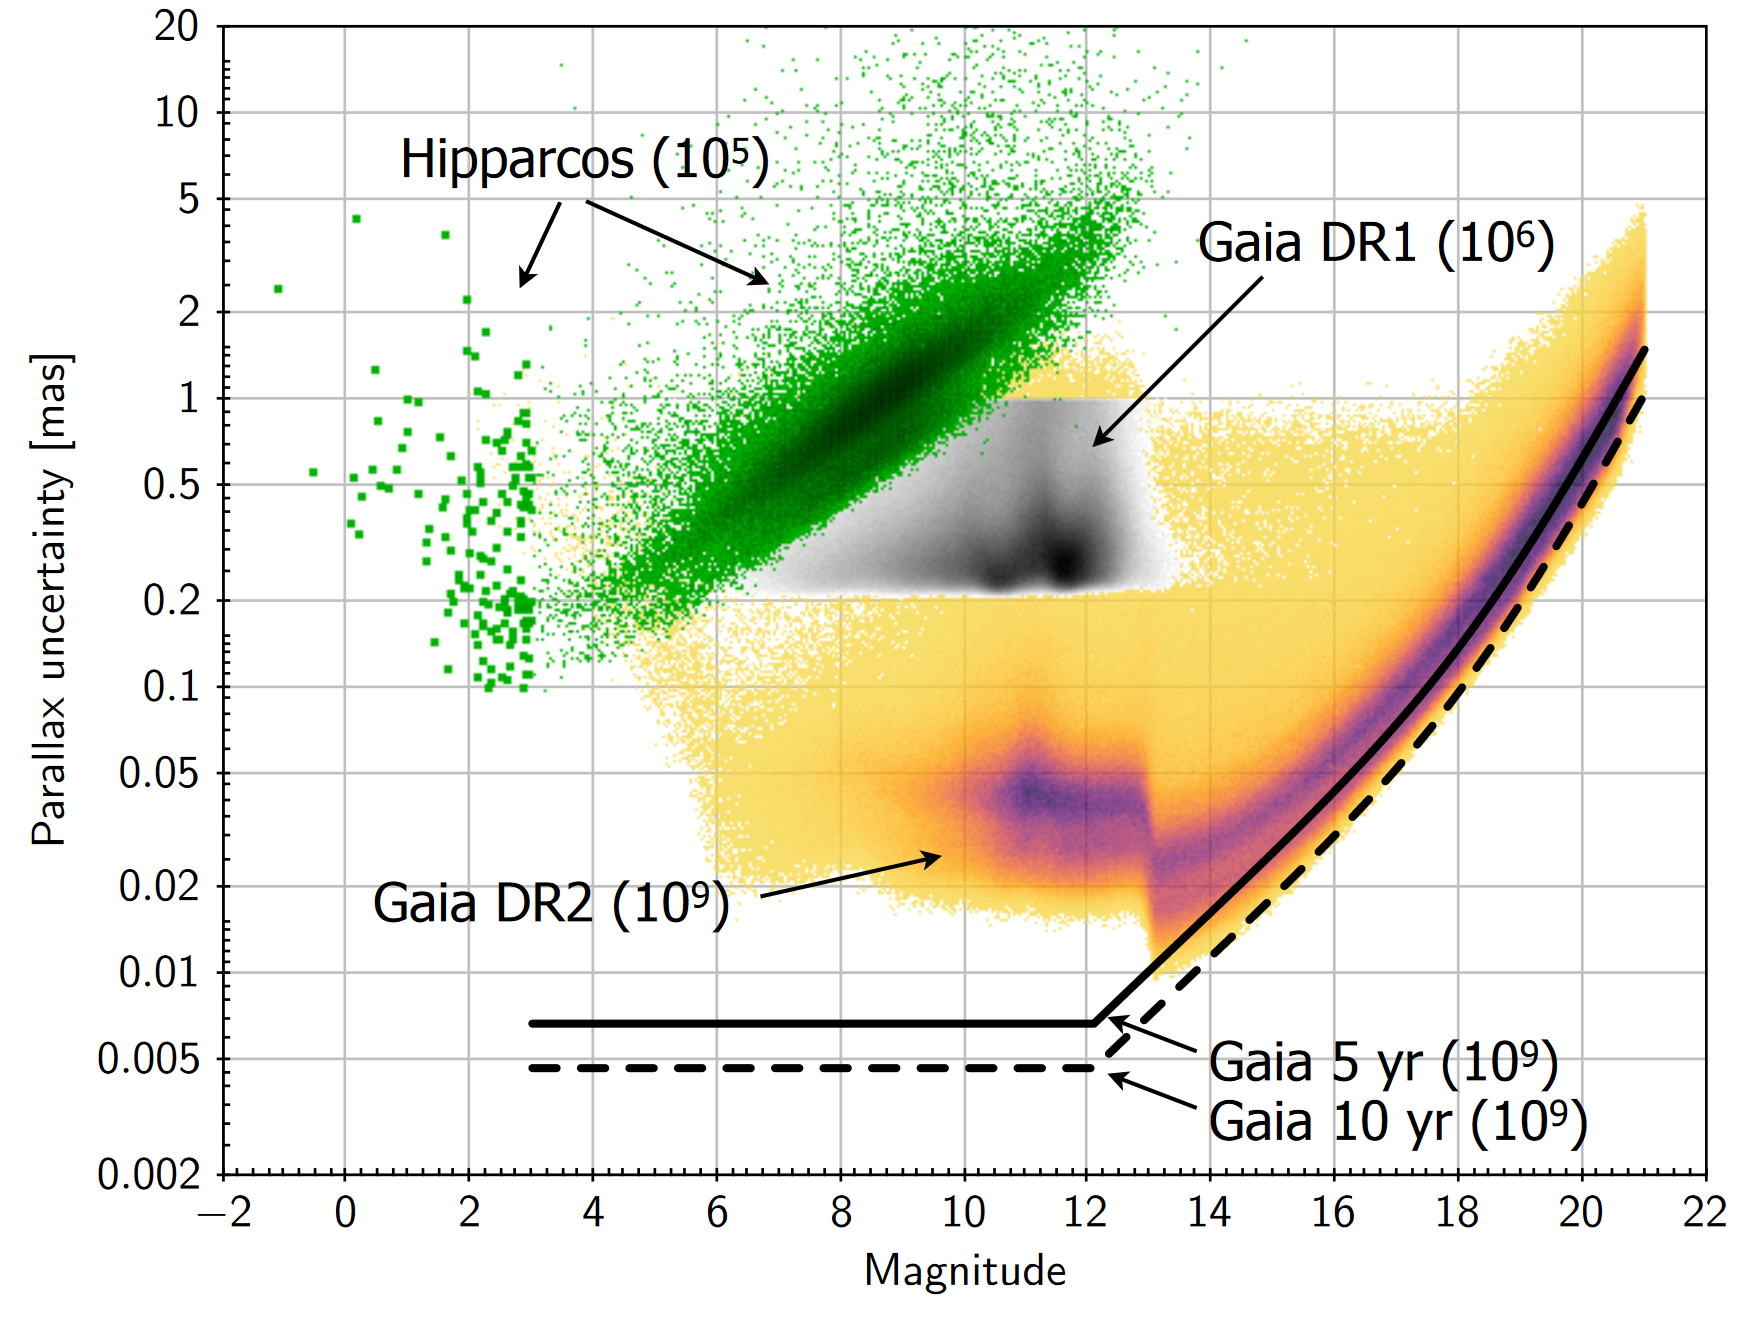
\includegraphics[width=\textwidth]{fig/c1/gaia_dr2_astrometry.png}
	\caption[Comparison between the astrometric accuracy for Hipparcos, Gaia, and future Gaia data releases]{Comparison between the astrometric accuracy for all sources in the final data release of Hipparcos, \gaia\ DR1, and \gaia\ DR2. The predicted accuracy of future data releases using 5 and 10 years of data is shown by the solid and dashed lines respectively. \emph{Credit}: \gaia\ DPAC.}
	\label{fig:intro:history:gaia_accuracy}
\end{figure}

Figure~\ref{fig:intro:history:gaia_accuracy} shows a comparison of the parallax uncertainty of \gaia\ data against data from the \emph{Hipparcos} satellite. In just over 20 years, technology progressed far enough to allow \gaia\ to measure parallaxes for $10^4$ times as many stars at a projected eventual accuracy as much as $10^3$ times better than \emph{Hipparcos}.





% Plot of gaia astrometric tracks
\begin{figure}[tb]
	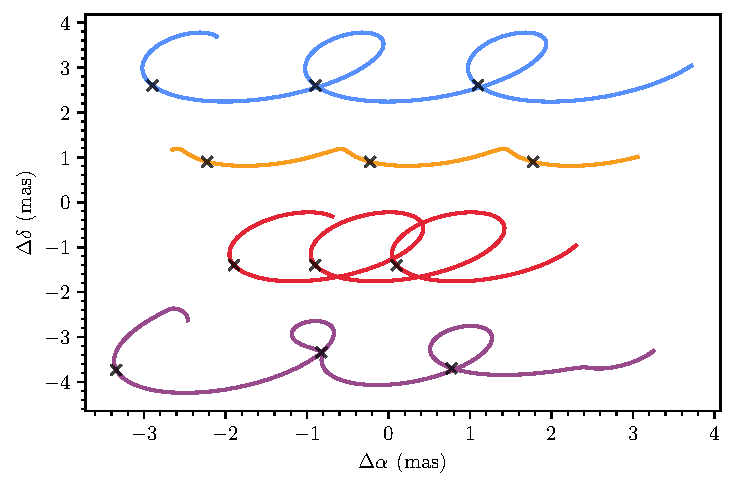
\includegraphics[width=\textwidth]{fig/c1/tracks.pdf}
	\caption[The predicted on-sky astrometric tracks of stars with different parameters]{The predicted on-sky astrometric tracks of stars with different parameters, generated using astromet \citep{penoyre_astrometric_2022}. All sources are at coordinates $\alpha,\,\beta=(0\degree,\,45\degree)$, but are offset in the $y$ direction for clarity of plotting. The first source has $\mu_{\alpha^*}=2$~masyr\textsuperscript{-1}, $\mu_{\delta}=0$, and is at a distance of 1~kpc. In the second example, the distance is quadrupled relative to the first. In the third example, the proper motion is halved relative to the first. In the final example, a binary with a period close to 1~yr, high eccentricity, and a low light ratio is added to the first example, producing a highly irregular track. The crosses denote the position of each source in one-year intervals.}
	\label{fig:intro:history:gaia_tracks}
\end{figure}

% Plot of hipparcos vs. gaia Blanco 1
\begin{figure}[tb]
	\centering
	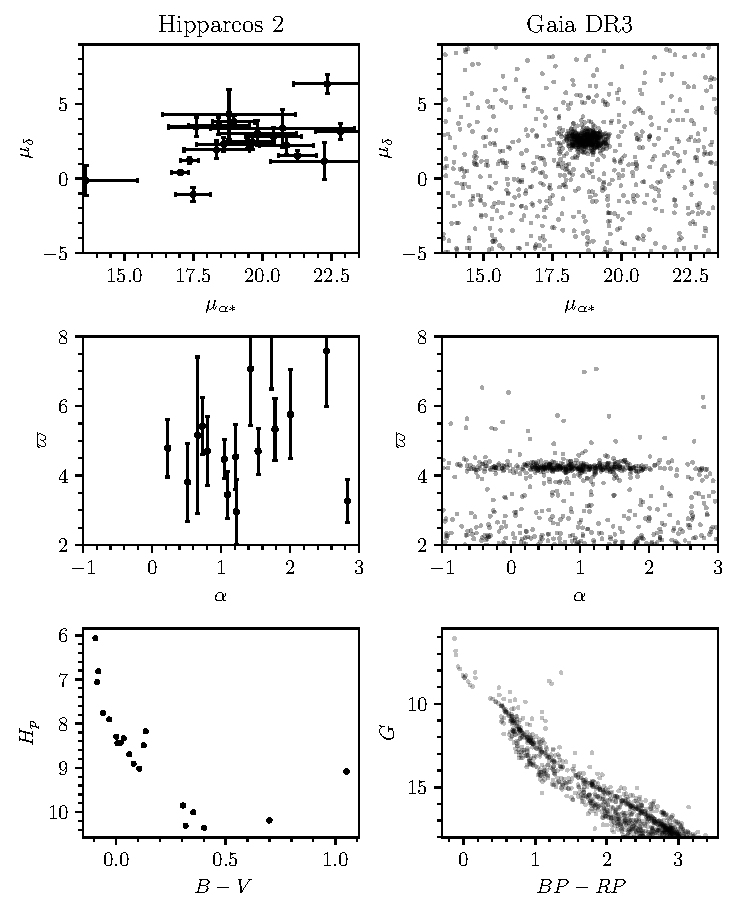
\includegraphics[width=0.9\textwidth]{fig/c1/gaia_hipparcos_oc_comparison.pdf}
	\caption[Comparison between the regions around the star cluster Blanco~1 in data from \emph{Hipparcos} and \gaia]{Comparison between the regions around the star cluster Blanco~1 in data from \emph{Hipparcos} and \gaia. \emph{Hipparcos}-2 data \citep{vanleeuwen_hipparcos_new_2007} is shown on the left and \gaia\ DR3 data \citep{gaia_collaboration_gaia_2022} is shown on the right. The top row shows proper motions, the middle row shows parallax as a function of right ascension, and the bottom row shows the CMD of the stars in each region. While \emph{Hipparcos} only sees a few dozen bright stars for the cluster, \gaia\ can detect up to 1000, and to a significantly higher degree of astrometric accuracy.}
	\label{fig:intro:history:gaia_blanco_1}
\end{figure}





% everything below this line is shit
\section{not sure where these bits will go yet}

\subsection{Common techniques in open cluster observations}
\label{sec:intro:history:techniques}
\subsubsection{Membership determination}

TODO. I honestly don't know enough here already lol

\subsubsection{Blind searches for open clusters}

TODO. Should lead in from the previous section.

\subsubsection{Isochrone fitting}

% Plot of CMDs of OCs
\begin{figure}[tb]
	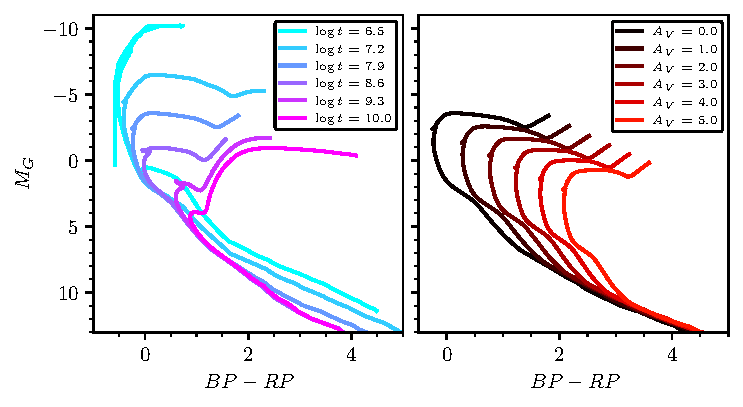
\includegraphics[width=\textwidth]{fig/c1/isochrones.pdf}
	\caption[A comparison between stellar isochrones of various different parameters.]{A comparison between stellar isochrones of various different parameters, derived from PARSEC stellar evolution models \citep{bressan_parsec_2012} and shown in \gaia\ photometric bands. \emph{Left:} isochrones of solar metallicity and zero extinction shown for six different ages. Most noticeably, as cluster age increases, the magnitude of the turn-off point decreases, with ever-more stars evolving into red giants and eventually reaching the end of their lives. The rest of the stars in the cluster also move down slightly, relaxing onto the main sequence as they age. \emph{Right:} the $\log t = 7.9$ isochrone from the left plotted at a range of different extinction values. Extinction reddens cluster stars as well as reducing their overall brightness. Extinction in \gaia\ photometry has a strong affect on the location of the turn-off point.}
	\label{fig:intro:history:isochrones}
\end{figure}

As discussed previously, CMDs are essential tools to derive many key parameters of a star cluster (Fig.~\ref{fig:intro:history:cmds}). The most common method to determine the age, extinction, and to a lesser extent the distance of a cluster is by fitting isochrones to cluster CMDs. An isochrone gives the predicted colour and luminosity of a population of stars with a range of masses given that the stars have the same age, extinction, composition and distance. Stellar isochrones are derived from stellar evolution models such as PARSEC \citep{bressan_parsec_2012} and are widely used in many areas of observational astronomy.

In practice, isochrones are difficult to fit, with age, extinction, distance and metallicity all being somewhat degenerate with one another. Figure~\ref{fig:intro:history:isochrones} shows the effect of varying age and extinction on stellar isochrones, with both age and extinction moving the location of the cluster turn-off point. Cluster distance merely shifts the isochrone up or down based on the cluster's distance modulus, although this is still slightly degenerate with age and extinction. Finally, the chemical composition of a cluster (most often parameterised with its metallicity $\left[\text{Fe}/\text{H}\right]$) has the smallest impact on cluster isochrones and is not shown, but will nevertheless slightly impact age and extinction determination.

Isochrone fitting is further complicated by the presence of other cluster features, such as the presence of a binary sequence due to unresolved binaries (see binary sequences in Fig~\ref{fig:intro:history:cmds}, showing a clear second line of stars sat slightly above the main cluster population).

Probably unsurprisingly, there are hence many methods used in the literature to fit isochrones to data. Particularly as computational power is a major hindrance to performing three or four-parameter fits with stellar isochrones, it was common to simply fit isochrones by hand (CITEME SOME EXAMPLES), which includes no robust uncertainty estimate and can open the door to human biases. The isochrones in \cite{kharchenko_global_2013} were fit using a hybrid method, with the authors fitting distances manually but then using $\chi^2$ minimisation to fit cluster age and reddening values. \cite{yen_reanalysis_2018} developed this methodology further to perform $\chi^2$ fitting of all cluster parameters. Finally, \cite{hippel_inverting_2006} created a full Bayesian methodology to fit isochrones to cluster CMDs, which is still used by works today in the \gaia\ era such as \cite{bossini_age_2019}.

By far the main flaw of cluster isochrone fitting is speed. Three or four-parameter fits using complicated stellar isochrones simply cannot be performed quickly, requiring significant amounts of computation time to complete in e.g. \cite{yen_reanalysis_2018}, making these key cluster parameters relatively time-intensive to derive using traditional isochrone fitting techniques.

\subsubsection{Radial profile fitting}

\subsubsection{Mass determination}


\subsection{Other important observations}
\label{sec:intro:history:other_obs}

\subsubsection{Binary stars in open clusters}

\subsubsection{Blue stragglers: some stars stay young for longer}

% Plot of blue stragglers
\begin{figure}[tb]
	\centering
	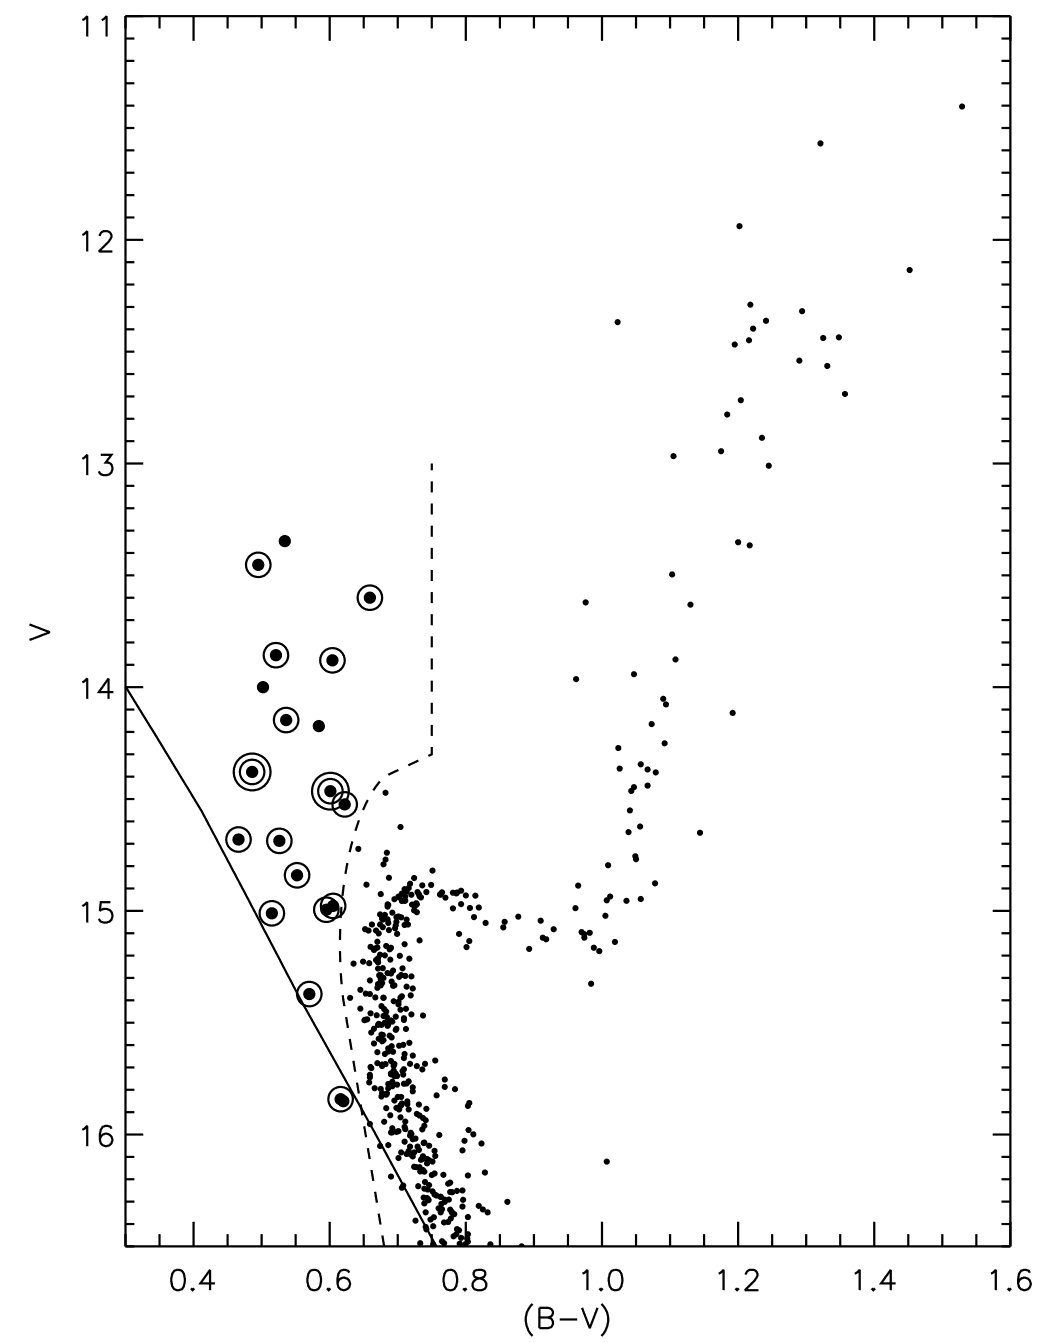
\includegraphics[width=0.6\textwidth]{fig/c1/ngc_188_blue_stragglers.png}
	\caption[TODO]{TODO}
	\label{fig:intro:history:blue_stragglers}
\end{figure}

\subsubsection{Extended main-sequence turn-offs (eMSTOs): not all OCs are perfect single populations}

% Plot of LMC cluster eMSTO
\begin{figure}[tb]
	\centering
	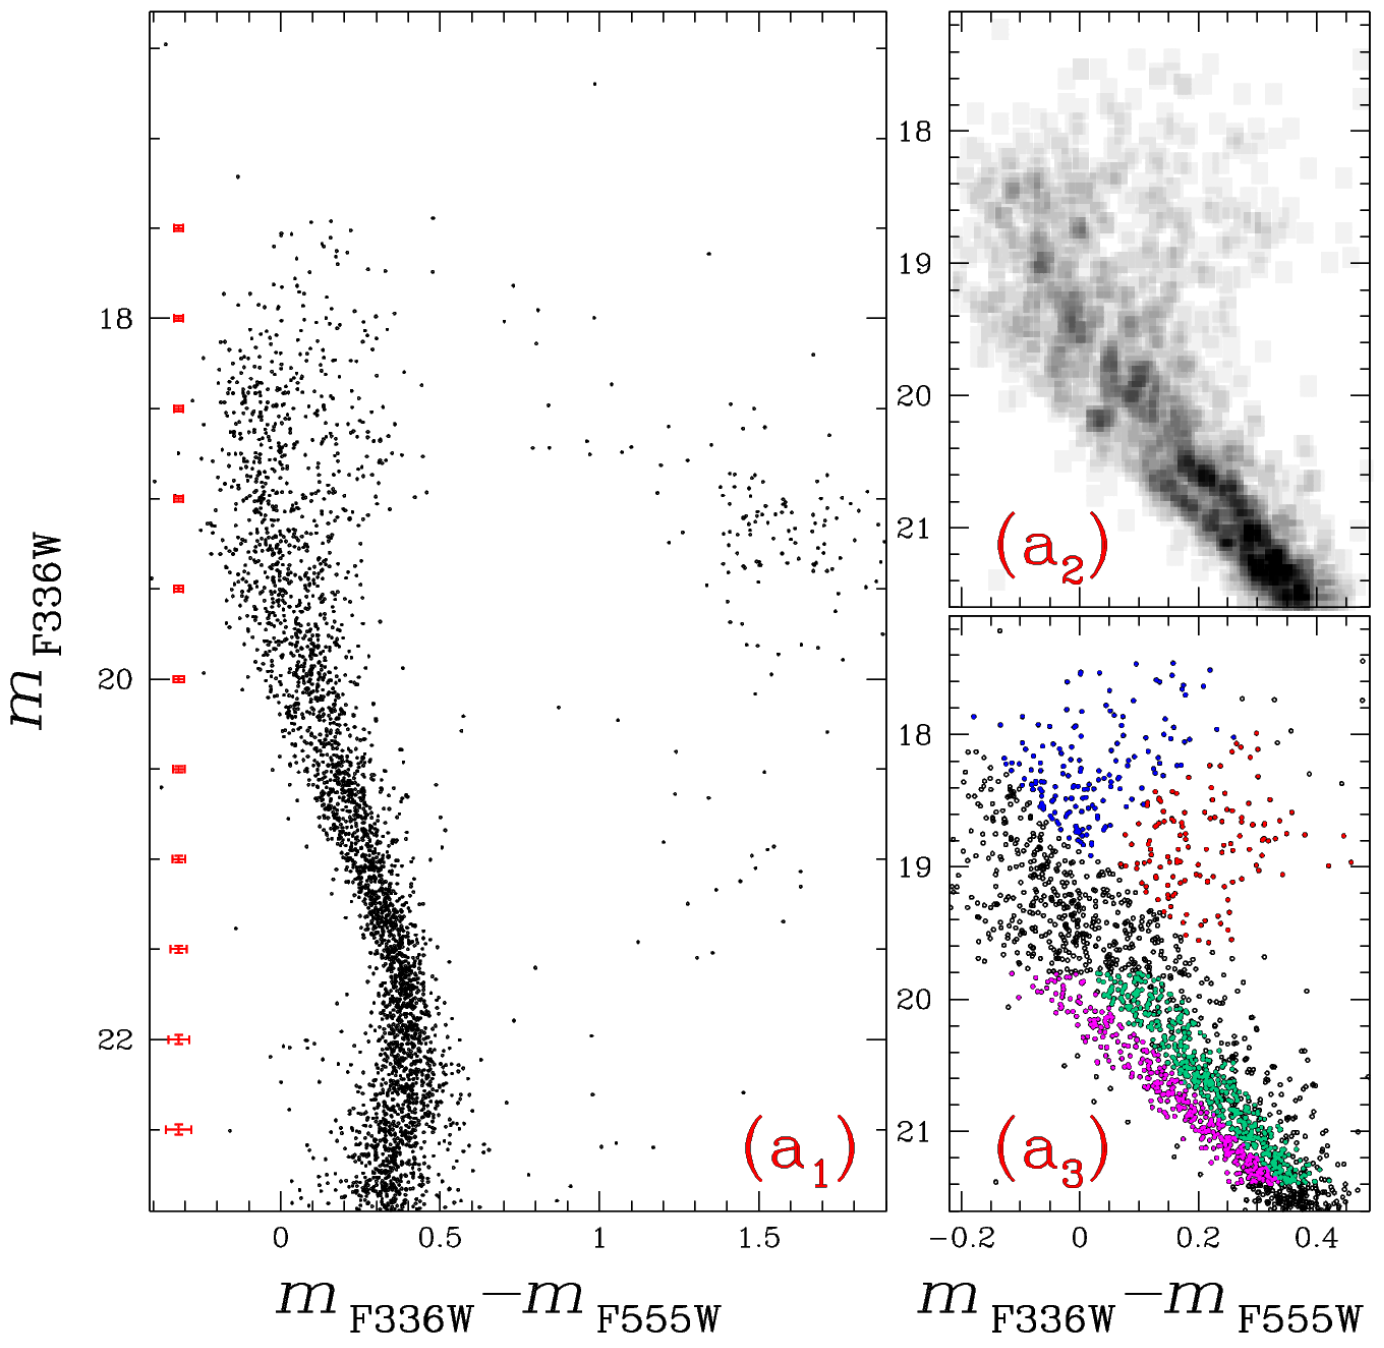
\includegraphics[width=0.7\textwidth]{fig/c1/emsto.png}
	\caption[TODO]{TODO}
	\label{fig:intro:history:emsto}
\end{figure}

\subsection{The pre-\gaia\ issues with the open cluster census}
\label{sec:intro:history:issues}






% ---------------------------------------
\section{The \gaia\ revolution in open cluster science}
\label{sec:intro:gaia}




\subsection{How \gaia\ has already revolutionised the open cluster census}
\label{sec:intro:gaia:census}


% Plot of reported OCs
\begin{figure}[tb]
	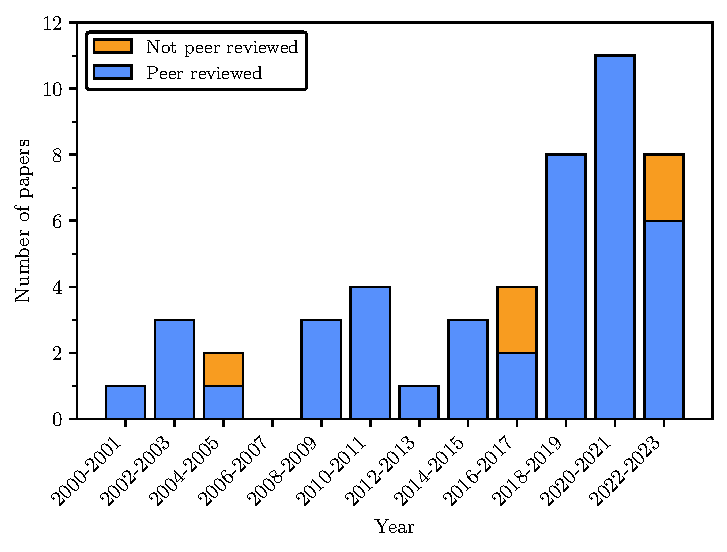
\includegraphics[width=\textwidth]{fig/c1/papers.pdf}
	\caption{TODO}
	\label{fig:intro:history:papers}
\end{figure}


\subsection{\gaia's brand new insights into open clusters}
\label{sec:intro:gaia:insights}

% Plot of Meingast+ tidal tails/comas
\begin{figure}[tb]
	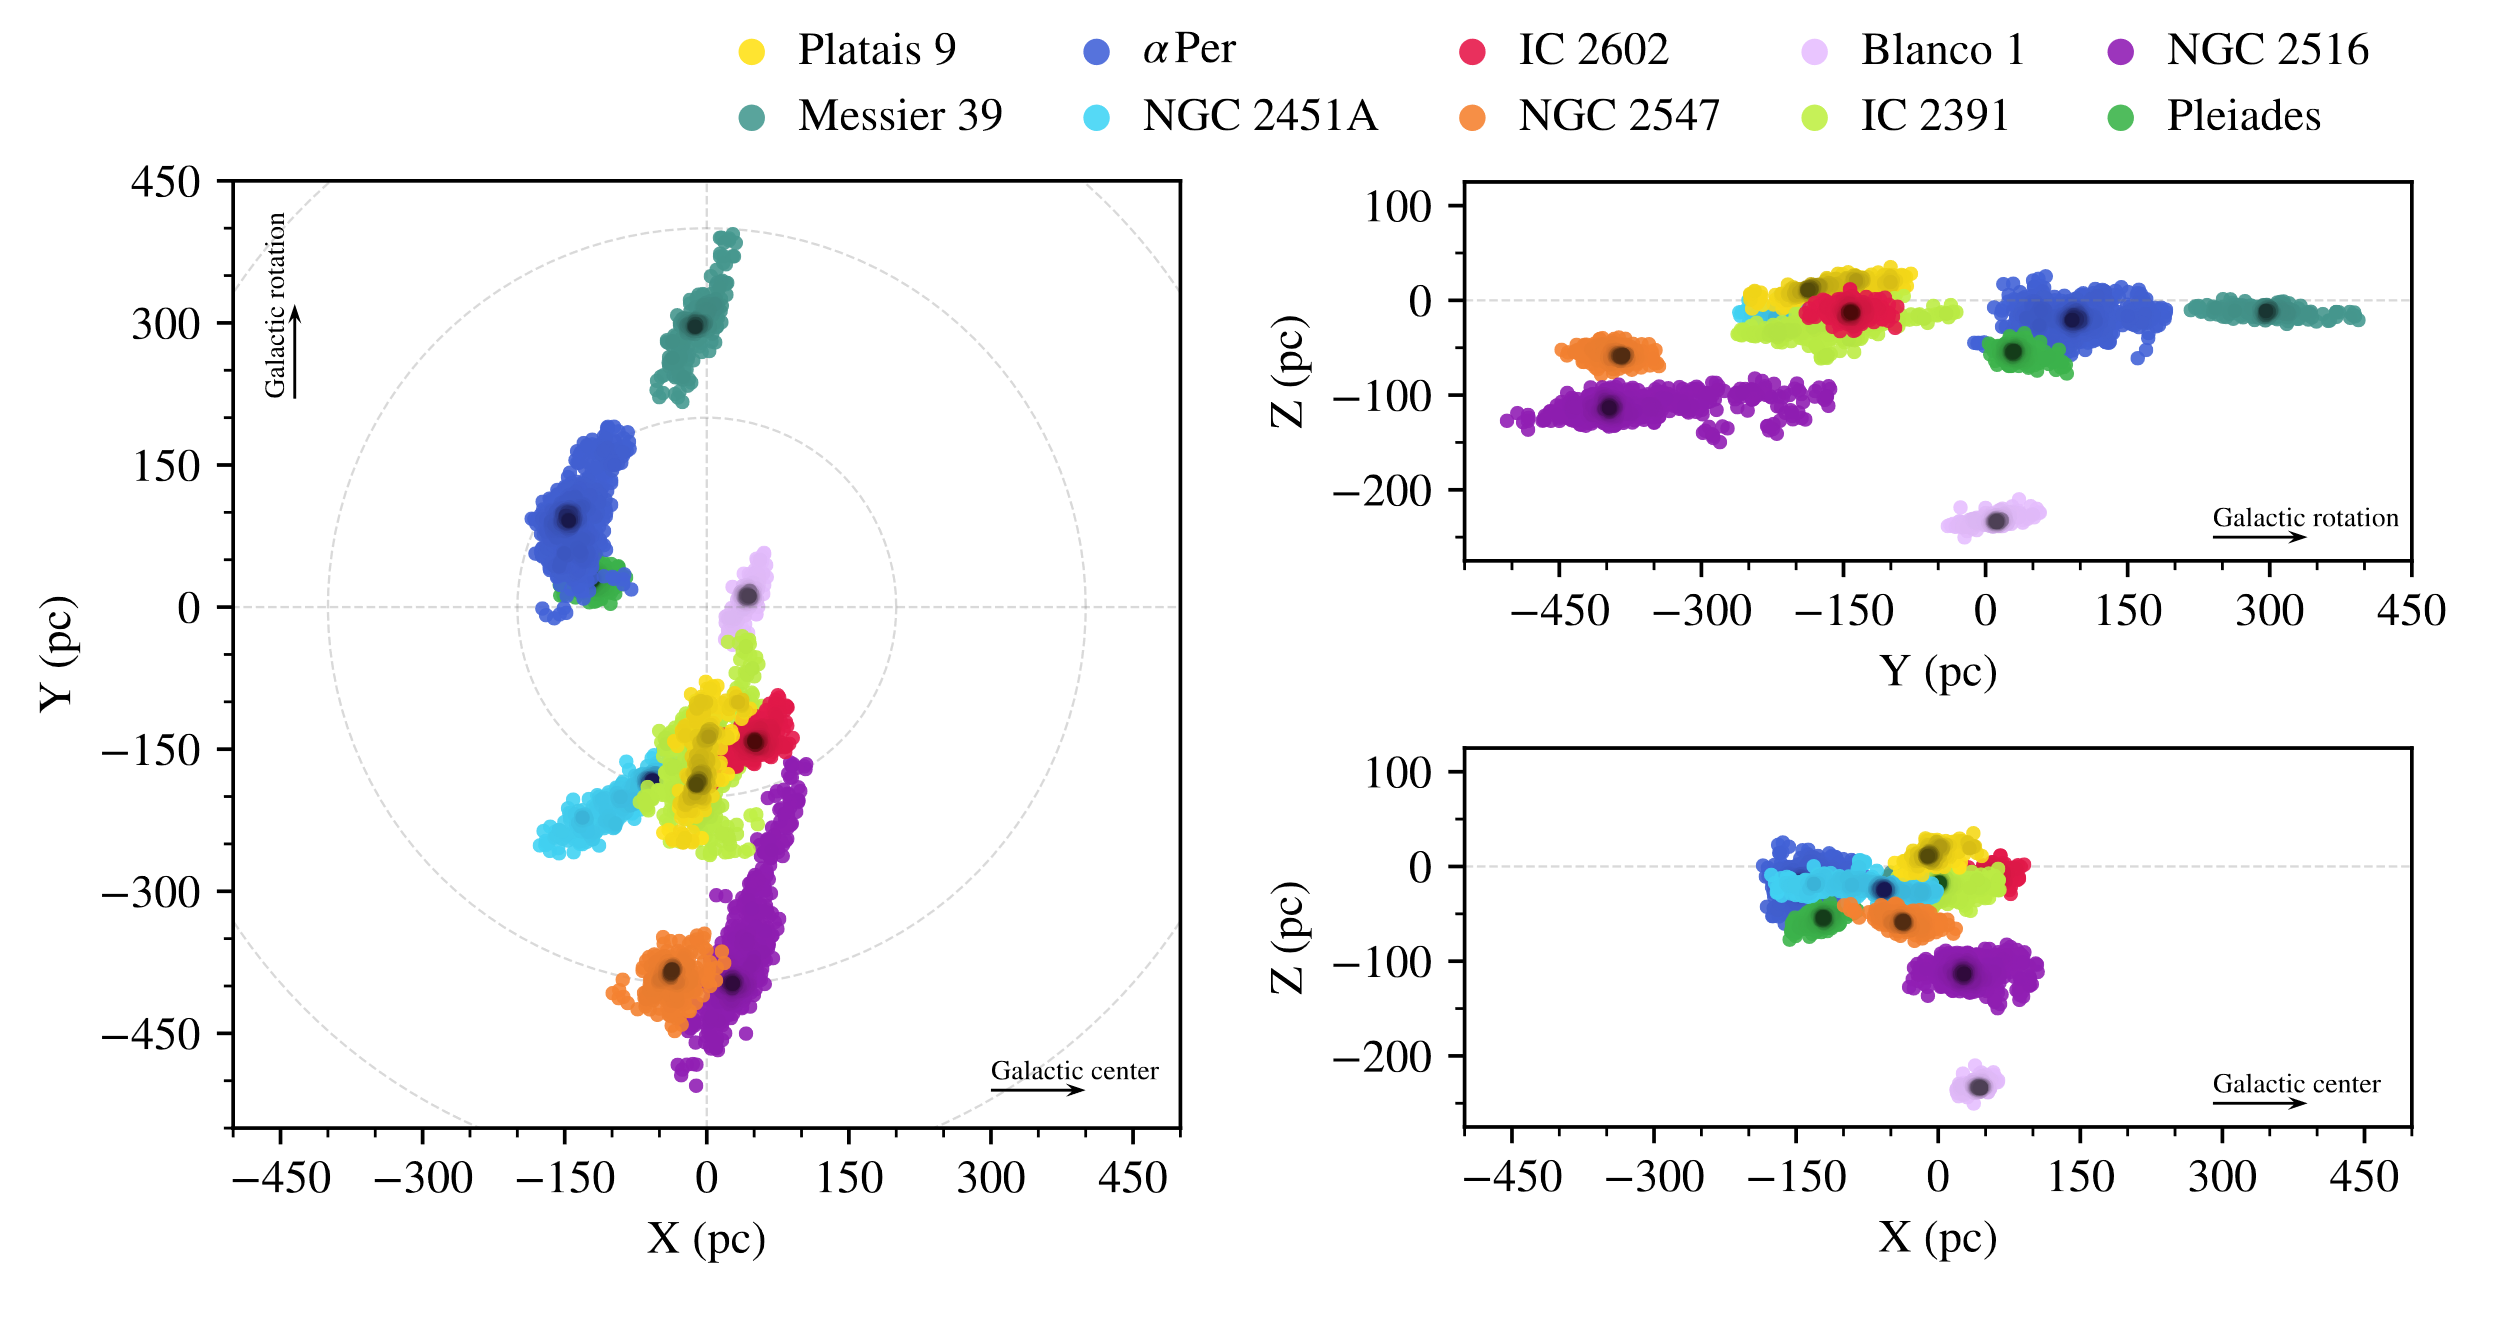
\includegraphics[width=\textwidth]{fig/c1/meingast_tidal_tails.png}
	\caption[TODO]{TODO}
	\label{fig:intro:gaia:comas}
\end{figure}

% Plot of OC spiral arm sort-of correlation
\begin{figure}[tb]
	\centering
	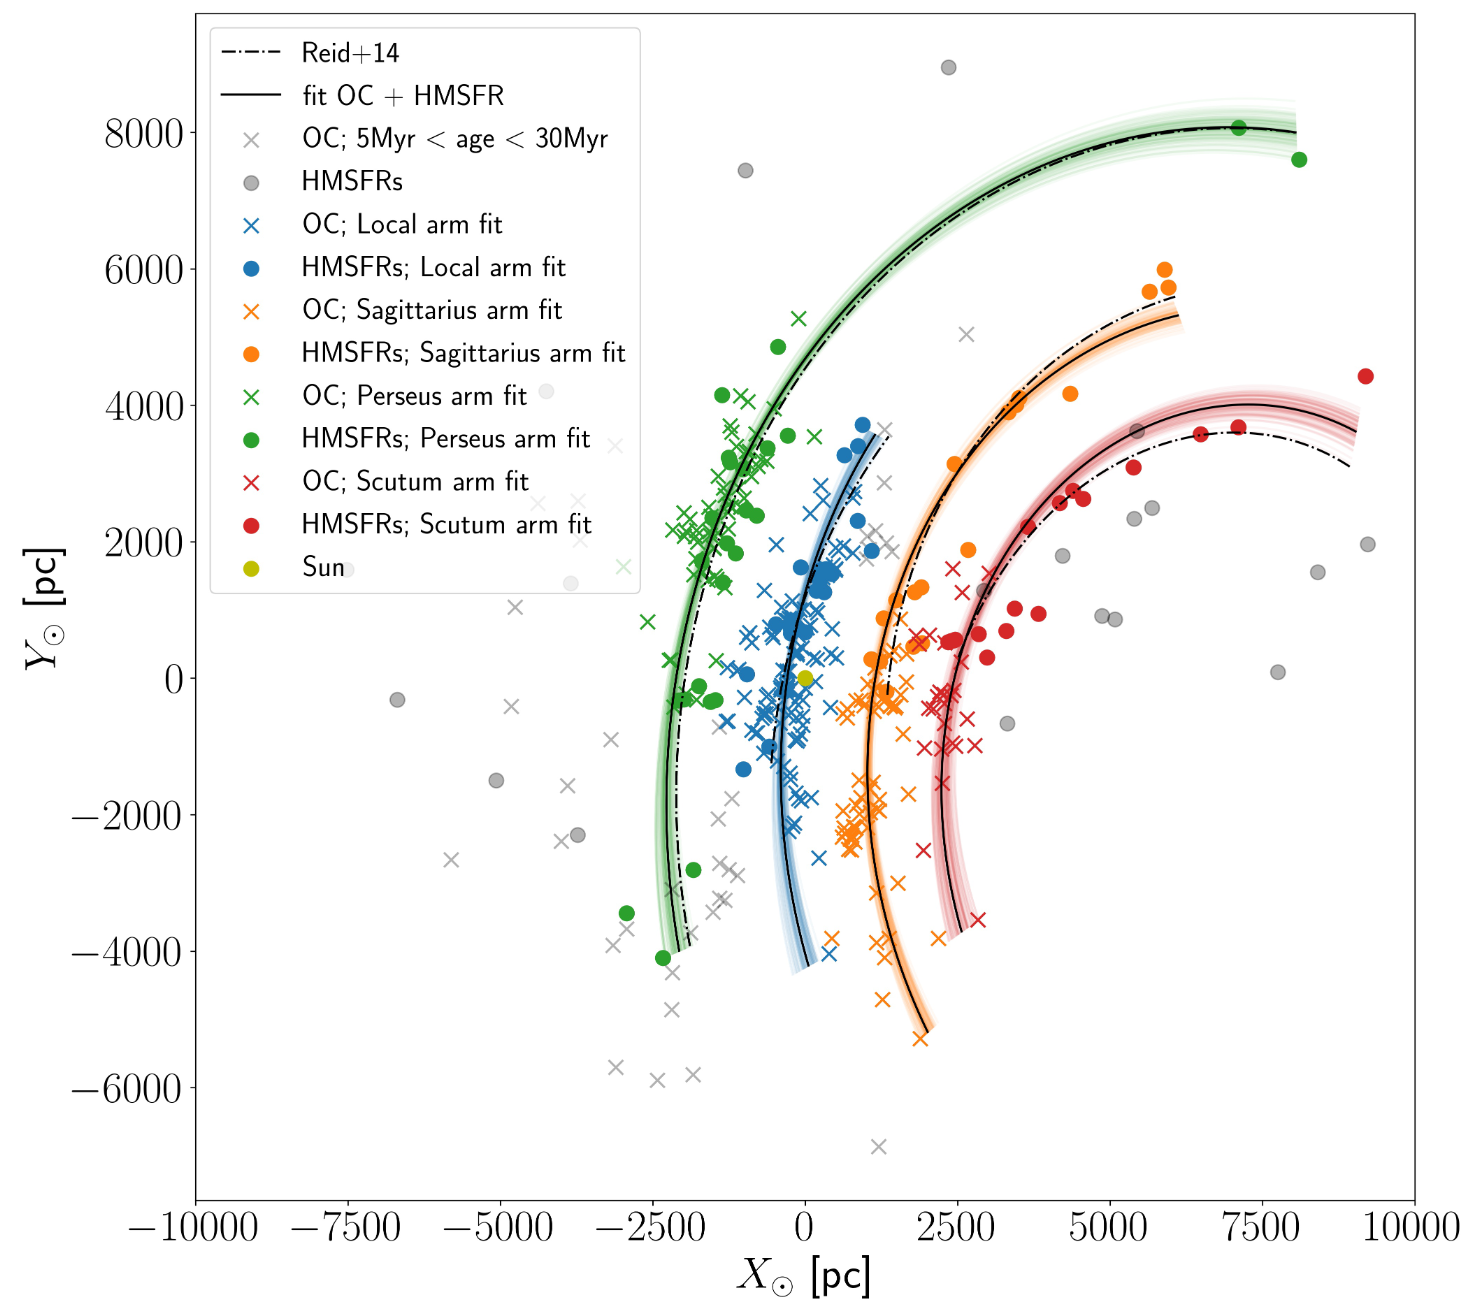
\includegraphics[width=0.8\textwidth]{fig/c1/spiral_arms.png}
	\caption[TODO]{TODO}
	\label{fig:intro:gaia:spiral}
\end{figure}


\subsection{The issues with open clusters in the \gaia\ era}
\label{sec:intro:gaia:issues}


% ---------------------------------------
\section{Some theoretical background into star clusters}
\label{sec:intro:theory}

\subsection{Radial profiles}
\label{sec:intro:theory:profile}


\subsection{Dynamics}
\label{sec:intro:theory:dynamics}


\subsection{Timescales}
\label{sec:intro:theory:timescales}


\subsection{Formation, evolution and destruction}
\label{sec:intro:theory:evolution}

% Plot of feedback vs. virial ratio
\begin{figure}[tb]
	\centering
	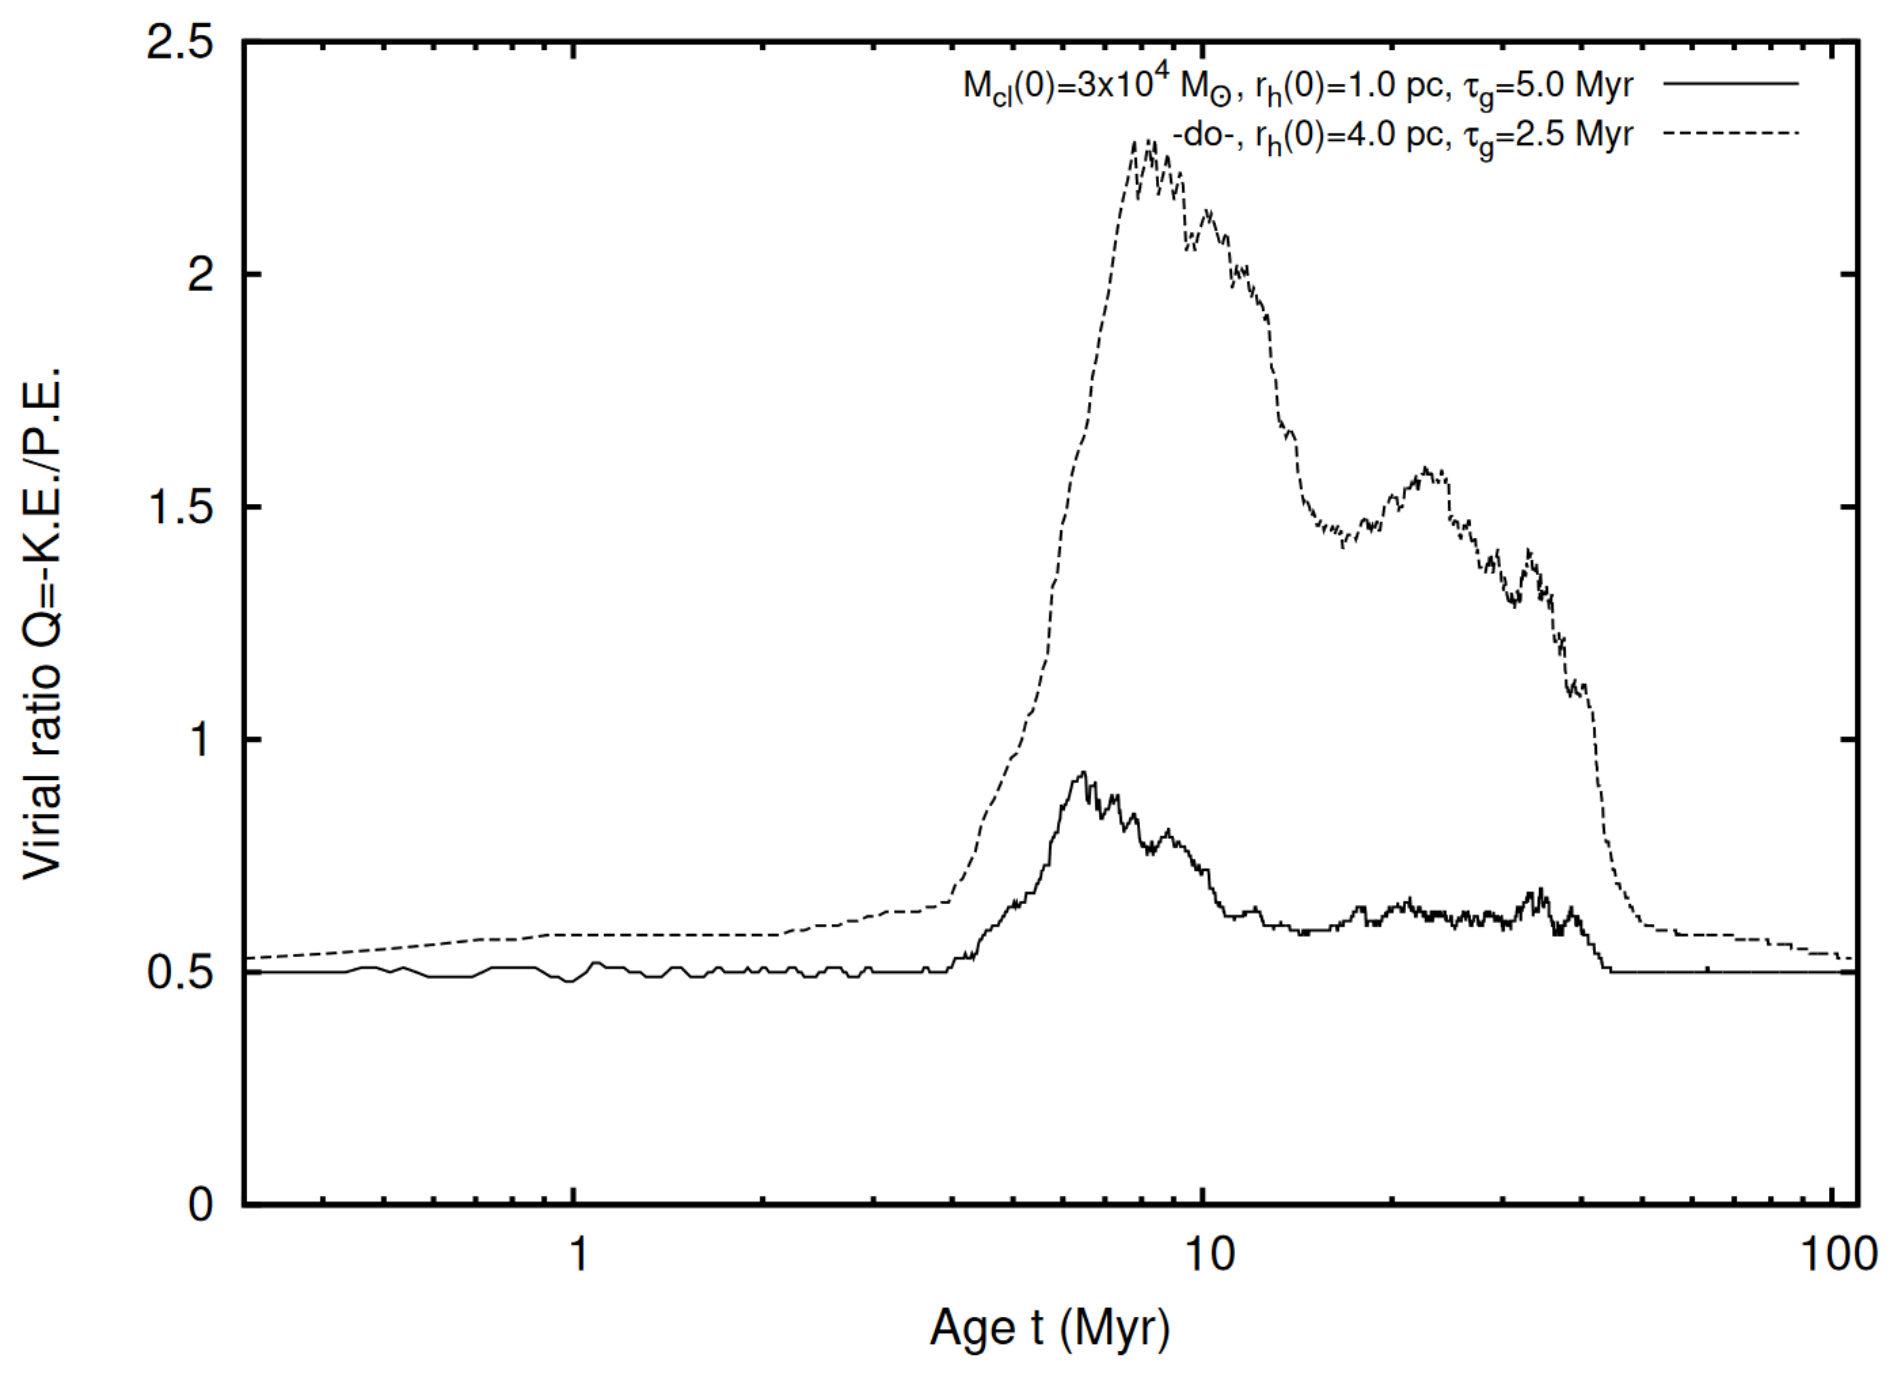
\includegraphics[width=0.8\textwidth]{fig/c1/virialisation_placid_gas_expulsion.png}
	\caption[TODO]{TODO}
	\label{fig:intro:theory:feedback}
\end{figure}


% ---------------------------------------
\section{Thesis structure}
\label{sec:intro:structure}

\textbf{Chapter \ref{sec:intro}} \\[0.2em]
\blindtext

\textbf{Chapter \ref{sec:intro}} \\[0.2em]
\blindtext

\textbf{Chapter \ref{sec:intro}} \\[0.2em]
\blindtext

\textbf{Chapter \ref{sec:intro}} \\[0.2em]
\blindtext

\textbf{Chapter \ref{sec:intro}} \\[0.2em]
\blindtext
